\begin{figure}
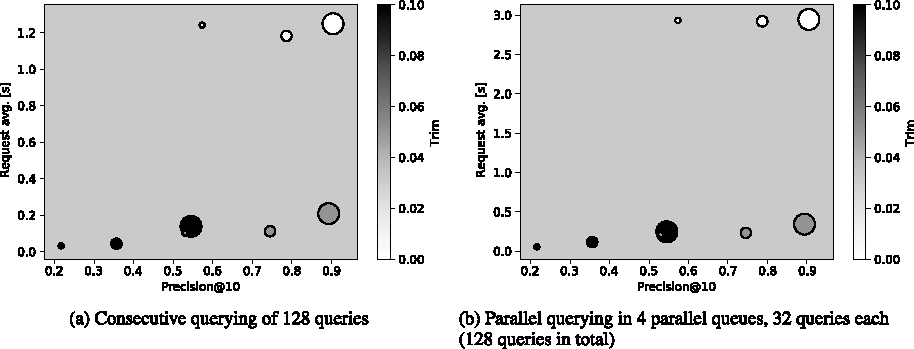
\includegraphics{scaletext-speed}
\vspace{-0.5cm}
\caption
  [The impact of removing unimportant features in our encoding and setting the
   number of results that are retrieved and reranked in our information
   retrieval system on its speed and accuracy]%
  {The impact of removing unimportant features (\emph{trim}) in our encoding and
   setting the number of results that are retrieved and reranked (\emph{page}) in
   our information retrieval system on its speed and accuracy: The
   $x$-axis shows the accuracy, the $y$-axis shows the speed, the point size
   shows the number of retrieved results (20, 80, and 320), and the color shows
   the number of removed features from none (white) to all with value below 0.1
   (black). Reproduced with permission. \cite[Figure 2]{rygl2017semantic}}
\label{fig:dense-retrieval-in-inverted-indices-speed}
\end{figure}
